\documentclass[bigtut]{tutorial}\usepackage[]{graphicx}\usepackage[]{color}
%% maxwidth is the original width if it is less than linewidth
%% otherwise use linewidth (to make sure the graphics do not exceed the margin)
\makeatletter
\def\maxwidth{ %
  \ifdim\Gin@nat@width>\linewidth
    \linewidth
  \else
    \Gin@nat@width
  \fi
}
\makeatother

\definecolor{fgcolor}{rgb}{0.345, 0.345, 0.345}
\newcommand{\hlnum}[1]{\textcolor[rgb]{0.686,0.059,0.569}{#1}}%
\newcommand{\hlstr}[1]{\textcolor[rgb]{0.192,0.494,0.8}{#1}}%
\newcommand{\hlcom}[1]{\textcolor[rgb]{0.678,0.584,0.686}{\textit{#1}}}%
\newcommand{\hlopt}[1]{\textcolor[rgb]{0,0,0}{#1}}%
\newcommand{\hlstd}[1]{\textcolor[rgb]{0.345,0.345,0.345}{#1}}%
\newcommand{\hlkwa}[1]{\textcolor[rgb]{0.161,0.373,0.58}{\textbf{#1}}}%
\newcommand{\hlkwb}[1]{\textcolor[rgb]{0.69,0.353,0.396}{#1}}%
\newcommand{\hlkwc}[1]{\textcolor[rgb]{0.333,0.667,0.333}{#1}}%
\newcommand{\hlkwd}[1]{\textcolor[rgb]{0.737,0.353,0.396}{\textbf{#1}}}%
\let\hlipl\hlkwb

\usepackage{framed}
\makeatletter
\newenvironment{kframe}{%
 \def\at@end@of@kframe{}%
 \ifinner\ifhmode%
  \def\at@end@of@kframe{\end{minipage}}%
  \begin{minipage}{\columnwidth}%
 \fi\fi%
 \def\FrameCommand##1{\hskip\@totalleftmargin \hskip-\fboxsep
 \colorbox{shadecolor}{##1}\hskip-\fboxsep
     % There is no \\@totalrightmargin, so:
     \hskip-\linewidth \hskip-\@totalleftmargin \hskip\columnwidth}%
 \MakeFramed {\advance\hsize-\width
   \@totalleftmargin\z@ \linewidth\hsize
   \@setminipage}}%
 {\par\unskip\endMakeFramed%
 \at@end@of@kframe}
\makeatother

\definecolor{shadecolor}{rgb}{.97, .97, .97}
\definecolor{messagecolor}{rgb}{0, 0, 0}
\definecolor{warningcolor}{rgb}{1, 0, 1}
\definecolor{errorcolor}{rgb}{1, 0, 0}
\newenvironment{knitrout}{}{} % an empty environment to be redefined in TeX

\usepackage{alltt}
\unitcode{MATH1005}
        \unitname{Statistics}
        \semester{Summer/WinterSemester2}
        \sheetnumber4

\usepackage{graphicx}
\withsolutions
\IfFileExists{upquote.sty}{\usepackage{upquote}}{}
\begin{document}
\lettersfirst

\begin{tutorial}

%\begin{displaybox}
%This tutorial explores bivariate data.  \\
%Most of this week's tutorial class will consist of the Report 1 presentations.  \\
%Complete the rest of the tutorial questions at home. \\
%\end{displaybox}

\begin{center}
\begin{tabular}{| ll |} \hline
& \\
{\bf Bivariate Data} & \\
For paired observations $\{ (x_i,y_i) \}$  & for $i=1,\ldots,n$ \\
& \\
summary statistics &   $S_{xy} = \sum_{i=1}^n x_iy_i -  \frac{1}{n} \Bigl( \sum_{i=1}^nx_i \Bigr)  \Bigl( \sum_{i=1}^ny_i\Bigr) $    \\
& $S_{xx} = \sum_{i=1}^n x_i^2 - \frac{1}{n} \Bigl(\sum_{i=1}^n x_i\Bigr)^2  = (n-1)s_{x}^2$       \\ 
& $S_{yy} = \sum_{i=1}^n y_i^2 - \frac{1}{n} \Bigl(\sum_{i=1}^n y_i\Bigr)^2$  \\
least squares regression line & $\hat{y}=a + bx$ \\
& where $a =\bar y - b \bar x$ and $b =\frac{S_{xy}}{S_{xx}}$ \\
correlation coefficient &  $r =\frac{S_{xy}}{\sqrt{S_{xx}S_{yy}}} = b \frac{s_x}{s_y}$ \\ 
& \\ 
proportion of variability &  $r^2$ \\ 
& \\ \hline
\end{tabular}
\end{center}

\vspace{.5cm}
\begin{questions}


\question Olympic Female 100m Sprint Times \\

The following data is race times for the 100m sprint by female athletes from 1928 (Amsterdam) to 2012 (London).

\begin{knitrout}
\definecolor{shadecolor}{rgb}{0.969, 0.969, 0.969}\color{fgcolor}\begin{kframe}
\begin{alltt}
\hlstd{Olympics100mW} \hlkwb{<-} \hlkwd{read.csv}\hlstd{(}\hlstr{"http://www.maths.usyd.edu.au/u/UG/JM/MATH1005/r/StatsData/
                          Olympics100mW.csv"}\hlstd{)}
\end{alltt}
\end{kframe}
\end{knitrout}

\vspace{.5cm}
\begin{parts}

\item What variables are recorded?
\begin{knitrout}
\definecolor{shadecolor}{rgb}{0.969, 0.969, 0.969}\color{fgcolor}\begin{kframe}
\begin{alltt}
\hlkwd{dim}\hlstd{(Olympics100mW)}
\hlkwd{names}\hlstd{(Olympics100mW)}
\end{alltt}
\end{kframe}
\end{knitrout}

\vspace{.5cm}
\item Who is the reigning champion? At which Olympics did she run and for what country?

\begin{knitrout}
\definecolor{shadecolor}{rgb}{0.969, 0.969, 0.969}\color{fgcolor}\begin{kframe}
\begin{alltt}
\hlstd{Result} \hlkwb{<-} \hlstd{Olympics100mW}\hlopt{$}\hlstd{Result}
\hlkwd{sort}\hlstd{(Result)}
\hlkwd{min}\hlstd{(Result)}
\end{alltt}
\end{kframe}
\end{knitrout}

\vspace{.5cm}
\item Are there any unusual times?
\begin{knitrout}
\definecolor{shadecolor}{rgb}{0.969, 0.969, 0.969}\color{fgcolor}\begin{kframe}
\begin{alltt}
\hlkwd{hist}\hlstd{(Result)}
\hlkwd{boxplot}\hlstd{(Result)}
\end{alltt}
\end{kframe}
\end{knitrout}

\vspace{.5cm}
\item Produce a scatter plot for the Results ($y$) vs Year ($x$). Does it suggest a linear regression might be appropriate?

\begin{knitrout}
\definecolor{shadecolor}{rgb}{0.969, 0.969, 0.969}\color{fgcolor}\begin{kframe}
\begin{alltt}
\hlstd{Year} \hlkwb{<-} \hlstd{Olympics100mW}\hlopt{$}\hlstd{Year}
\hlkwd{plot}\hlstd{(Year,Result)}
\end{alltt}
\end{kframe}
\end{knitrout}

Note:  Plots can be customised:
\begin{knitrout}
\definecolor{shadecolor}{rgb}{0.969, 0.969, 0.969}\color{fgcolor}\begin{kframe}
\begin{alltt}
\hlkwd{help}\hlstd{(plot)}
\hlkwd{plot}\hlstd{(Year,Result,}\hlkwc{main}\hlstd{=}\hlstr{"Olympics 1928-2012"}\hlstd{,}\hlkwc{xlab}\hlstd{=}\hlstr{"Years"}\hlstd{,}\hlkwc{ylab}\hlstd{=}\hlstr{"Results (s)"}\hlstd{,}
     \hlkwc{col}\hlstd{=}\hlstr{"blue"}\hlstd{,}\hlkwc{pch}\hlstd{=}\hlnum{6}\hlstd{)}
\end{alltt}
\end{kframe}
\end{knitrout}

A list of the \texttt{pch} (plotting characters) is here: 
{\tiny http://www.statmethods.net/advgraphs/parameters.html} 


\vspace{.5cm}
\item Fit a linear regression line.
\begin{knitrout}
\definecolor{shadecolor}{rgb}{0.969, 0.969, 0.969}\color{fgcolor}\begin{kframe}
\begin{alltt}
\hlstd{fit} \hlkwb{<-} \hlkwd{lm}\hlstd{(Result} \hlopt{~} \hlstd{Year)}
\hlstd{fit}
\hlkwd{abline}\hlstd{(fit)}   \hlcom{#This adds the LRline to the scatterplot}
\end{alltt}
\end{kframe}
\end{knitrout}

\vspace{.5cm}
\item Produce a regression plot. Does it suggest the linear regression is appropriate?
\begin{knitrout}
\definecolor{shadecolor}{rgb}{0.969, 0.969, 0.969}\color{fgcolor}\begin{kframe}
\begin{alltt}
\hlkwd{plot}\hlstd{(Year,fit}\hlopt{$}\hlstd{residuals)}
\hlkwd{abline}\hlstd{(}\hlkwc{h} \hlstd{=} \hlnum{0}\hlstd{)}
\end{alltt}
\end{kframe}
\end{knitrout}

\vspace{.5cm}
\item What is the correlation coefficient and proportion of variation?
\begin{knitrout}
\definecolor{shadecolor}{rgb}{0.969, 0.969, 0.969}\color{fgcolor}\begin{kframe}
\begin{alltt}
\hlkwd{cor}\hlstd{(Year,Result)}
\hlkwd{cor}\hlstd{(Year,Result)}\hlopt{^}\hlnum{2}
\end{alltt}
\end{kframe}
\end{knitrout}

\vspace{.5cm}
\item If the trend continues, what would you predict the result will be at the 2016 Rio Olympics?

\begin{knitrout}
\definecolor{shadecolor}{rgb}{0.969, 0.969, 0.969}\color{fgcolor}\begin{kframe}
\begin{alltt}
\hlstd{a}\hlkwb{=} \hlstd{fit}\hlopt{$}\hlstd{coefficients[[}\hlnum{1}\hlstd{]]}
\hlstd{b}\hlkwb{=} \hlstd{fit}\hlopt{$}\hlstd{coefficients[[}\hlnum{2}\hlstd{]]}
\hlstd{yhat} \hlkwb{=} \hlstd{a}\hlopt{+} \hlstd{b}\hlopt{*}\hlstd{(}\hlnum{2016}\hlstd{)}
\hlstd{yhat}
\end{alltt}
\end{kframe}
\end{knitrout}
\end{parts}


\begin{solution}
The data consists of 60 athletes over 20 Olympics with 5 variables. The reigning champion is Florence Griffith-Joyner from the USA with a time of 10.54s at the 1988 Seoul Olympics. The boxplot shows no outliers (unusual results). The scatter plot indicates a linear regression might be appropriate which is further suggested by $r=-0.8736502$ and that 76\% of the variability of Results is explained by Years. The 2016 predicetd result is 10.61s which is still higher than Florence's record in 1988.
\end{solution} 


\question Sydney to Hobart Winning Race Times \\

The Sydney-Hobart yacht race is a 630 nautical mile ocean race which starts from Sydney Harbour on Boxing Day (December 26) and finishes several days later in Hobart. It is considered one of the most difficult yacht races in the world. The following data is the winning times from 1945 to 1993 (as they appeared in the Sydney Morning Herald on 24 December 1994) plus the winning times for 1994 to 1997. We will examine the relationship between the log(Time) ($y$) and Year ($x$).

\begin{knitrout}
\definecolor{shadecolor}{rgb}{0.969, 0.969, 0.969}\color{fgcolor}\begin{kframe}
\begin{alltt}
\hlstd{Race} \hlkwb{<-} \hlkwd{read.table}\hlstd{(}\hlstr{"http://www.statsci.org/data/oz/sydhob.txt"}\hlstd{,}\hlkwc{header}\hlstd{=T)}
\end{alltt}
\end{kframe}
\end{knitrout}

\vspace{.5cm}
\begin{parts}
\item What variables are recorded?
\begin{knitrout}
\definecolor{shadecolor}{rgb}{0.969, 0.969, 0.969}\color{fgcolor}\begin{kframe}
\begin{alltt}
\hlkwd{dim}\hlstd{(Race)}
\hlkwd{names}\hlstd{(Race)}
\end{alltt}
\end{kframe}
\end{knitrout}

\vspace{.5cm}
\item From this data, what is the best race time? Which year was it achieved and by what boat? Compare this to the best time ever by Wild Oats in 2012.
{\tiny {https://en.wikipedia.org/wiki/Sydney\_to\_Hobart\_Yacht\_Race}}

\begin{knitrout}
\definecolor{shadecolor}{rgb}{0.969, 0.969, 0.969}\color{fgcolor}\begin{kframe}
\begin{alltt}
\hlstd{Time} \hlkwb{<-} \hlstd{Race}\hlopt{$}\hlstd{Time}
\hlkwd{min}\hlstd{(Time)}
\end{alltt}
\end{kframe}
\end{knitrout}

\vspace{.5cm}
\item Are there any unusual times? What was the time and year and boat?
\begin{knitrout}
\definecolor{shadecolor}{rgb}{0.969, 0.969, 0.969}\color{fgcolor}\begin{kframe}
\begin{alltt}
\hlkwd{boxplot}\hlstd{(Time)}
\end{alltt}
\end{kframe}
\end{knitrout}

\vspace{.5cm}
\item Take a logarithm transformation of Time to get rid of the outlier, and use this as your subsequent $y$ variable.
\begin{knitrout}
\definecolor{shadecolor}{rgb}{0.969, 0.969, 0.969}\color{fgcolor}\begin{kframe}
\begin{alltt}
\hlstd{LTime} \hlkwb{<-} \hlkwd{log}\hlstd{(Time)}
\hlkwd{boxplot}\hlstd{(LTime)}
\end{alltt}
\end{kframe}
\end{knitrout}


\vspace{.5cm}
\item Produce a scatter plot for LTime ($y$) and Year ($x$). Does it suggest a linear regression might be appropriate?

\begin{knitrout}
\definecolor{shadecolor}{rgb}{0.969, 0.969, 0.969}\color{fgcolor}\begin{kframe}
\begin{alltt}
\hlstd{Year} \hlkwb{<-} \hlstd{Race}\hlopt{$}\hlstd{Year}
\hlkwd{plot}\hlstd{(Year,LTime,} \hlkwc{ylab}\hlstd{=}\hlstr{"Log(Time)"}\hlstd{,}\hlkwc{main}\hlstd{=}\hlstr{"Sydney-Hobart Race Times 1945-1997"}\hlstd{)}
\end{alltt}
\end{kframe}
\end{knitrout}

\vspace{.5cm}
\item Fit a linear regression line.
\begin{knitrout}
\definecolor{shadecolor}{rgb}{0.969, 0.969, 0.969}\color{fgcolor}\begin{kframe}
\begin{alltt}
\hlstd{fit} \hlkwb{<-} \hlkwd{lm}\hlstd{(LTime} \hlopt{~} \hlstd{Year)}
\hlstd{fit}
\hlkwd{abline}\hlstd{(fit,} \hlkwc{col}\hlstd{=}\hlstr{"red"}\hlstd{,} \hlkwc{lwd}\hlstd{=}\hlnum{2}\hlstd{)}
\hlkwd{abline}\hlstd{(}\hlkwc{a}\hlstd{=}\hlnum{32.71984}\hlstd{,} \hlkwc{b}\hlstd{=}\hlopt{-}\hlnum{0.01224}\hlstd{,} \hlkwc{col}\hlstd{=}\hlstr{"blue"}\hlstd{,} \hlkwc{lwd}\hlstd{=}\hlnum{2}\hlstd{)}  \hlcom{## alternative method}
\end{alltt}
\end{kframe}
\end{knitrout}

\vspace{.5cm}
\item Produce a regression plot. Does it suggest the linear regression is appropriate?
\begin{knitrout}
\definecolor{shadecolor}{rgb}{0.969, 0.969, 0.969}\color{fgcolor}\begin{kframe}
\begin{alltt}
\hlkwd{plot}\hlstd{(Year,fit}\hlopt{$}\hlstd{residuals,} \hlkwc{ylab}\hlstd{=}\hlstr{"Residulals"}\hlstd{,} \hlkwc{main}\hlstd{=}\hlstr{"Residual Plot"}\hlstd{)}
\hlkwd{abline}\hlstd{(}\hlkwc{h} \hlstd{=} \hlnum{0}\hlstd{)}
\end{alltt}
\end{kframe}
\end{knitrout}

\vspace{.5cm}
\item What is the correlation coefficient and proportion of variation?
\begin{knitrout}
\definecolor{shadecolor}{rgb}{0.969, 0.969, 0.969}\color{fgcolor}\begin{kframe}
\begin{alltt}
\hlkwd{cor}\hlstd{(Year,LTime)}
\hlkwd{cor}\hlstd{(Year,LTime)}\hlopt{^}\hlnum{2}
\end{alltt}
\end{kframe}
\end{knitrout}

\vspace{.5cm}
\item Using the LSL, what would you predict the winning time to be in 2080? How does this warn us about extrapolation?

\end{parts}

\begin{solution}
The data consists of 53 wining race times with 5 variables. The reigning champion during these years was Morning Glory with a time of 3727.2mins in 1996. The best ever race time was in 2012 by Wild Oats: 2543.2mins (1 day, 18hr, 23mins, 12s)! The boxplot shows 1 outlier (9502mins in 1945 by Rani). The scatter plot indicates a linear regression might be appropriate. The correlation coefficient is -0.7918511 with proportion of variability of approx 63\%. \\

Using the LSL,
$\hat{log(y)} = 32.71984 -0.01224*x$.\\
So in 2080, $\hat{log(y)} = 32.71984 -0.01224*2080 = 7.26064$. \\
Hence, $\hat{y} = e^{7.26064} = 1423.167$, which is 0.988days. \\
Even though yachts are getting faster, it seems unlikely that the race could be completed in less than a day.
\end{solution} 


\vspace{.5cm}
\question
The following data has $r \approx -0.53$. Experiment with changing the data to decrease and increase the correlation coefficient.

\begin{knitrout}
\definecolor{shadecolor}{rgb}{0.969, 0.969, 0.969}\color{fgcolor}\begin{kframe}
\begin{alltt}
\hlstd{x}\hlkwb{=}\hlkwd{c}\hlstd{(}\hlnum{1}\hlstd{,}\hlnum{2}\hlstd{,}\hlnum{3}\hlstd{,}\hlnum{4}\hlstd{,}\hlnum{5}\hlstd{,}\hlnum{6}\hlstd{)}
\hlstd{y}\hlkwb{=}\hlkwd{c}\hlstd{(}\hlnum{2}\hlstd{,}\hlnum{6}\hlstd{,}\hlnum{5}\hlstd{,}\hlnum{5}\hlstd{,}\hlnum{3}\hlstd{,}\hlnum{8}\hlstd{)}
\hlkwd{plot}\hlstd{(x,y)}
\hlkwd{cor}\hlstd{(x,y)}
\end{alltt}
\end{kframe}
\end{knitrout}












\newpage
\hspace{-1cm} {\bf Extra Questions}

\question Traffic density and carbon monoxide concentration in Newtown  \\

Of environmental interest is the relation between carbon monoxide concentration and  traffic density.  The following table gives the traffic density (vehicles per hour to the nearest 500 vehicles) and carbon monoxide concentration (CO) in ppm for a particular street corner in Newtown. \\
Note the table reads as $(x_1,y_1)=(1.0,9),(x_2,y_2)=(1.0,6.8),\ldots(x_{12},y_{12})=(3.0,20.6) $ 
\vskip 2mm
\begin{center}
\begin{tabular}{|c|l|}  \hline
$x$: Traffic density (in thousands)&$y$: CO concentration (in ppm)\\ \hline
1.0&\phantom{1}9.0\,\, \phantom{1}6.8\,\, \phantom{1}7.7 \\
 1.5&\phantom{1}9.6\,\, \phantom{1}6.8\,\, 10.3\\
2.0&12.3\,\, 11.8\\
3.0&20.7\,\, 20.2\,\, 21.6\,\, 20.6 \\ \hline
\end{tabular}
\end{center}
\vskip 1mm

\vspace{.5cm}
Do parts (a)-(g) by hand.
\begin{parts}
\item Produce a scatter plot. Does a linear fit seem reasonable? \\

\part Calculate the summary statistics from  \\
$ \sum_{i=1}^{12} x_iy_i  = 361.05,   \sum_{i=1}^{12} x_i^2 =  53.75, \sum_{i=1}^{12} y_i^2 = 2449, \sum_{i=1}^{12} x_i  =   23.5,
 \sum_{i=1}^{12} y_i = 157.4$ \\

\part   Calculate the mean and variance of $x$ and $y$. \\

\part  Find the least squares regression line and correlation coefficient. What does $r$ suggest? \\

\part  What is the predicted CO concentration on a day with traffic density 2,500?  \\

\part  For the reading (2.0,12.3), what is the residual?  \\

\part  On a day with traffic density of 5,000, would it be appropriate to use the least squares regression line to predict the CO concentration?  Explain. \\

\part Now check your results using R.

\begin{knitrout}
\definecolor{shadecolor}{rgb}{0.969, 0.969, 0.969}\color{fgcolor}\begin{kframe}
\begin{alltt}
\hlstd{x}\hlkwb{=}\hlkwd{c}\hlstd{(}\hlnum{1}\hlstd{,}\hlnum{1}\hlstd{,}\hlnum{1}\hlstd{,}\hlnum{1.5}\hlstd{,}\hlnum{1.5}\hlstd{,}\hlnum{1.5}\hlstd{,}\hlnum{2}\hlstd{,}\hlnum{2}\hlstd{,}\hlnum{3}\hlstd{,}\hlnum{3}\hlstd{,}\hlnum{3}\hlstd{,}\hlnum{3}\hlstd{)}
\hlstd{y}\hlkwb{=}\hlkwd{c}\hlstd{(}\hlnum{9.0}\hlstd{,}\hlnum{6.8}\hlstd{,}\hlnum{7.7}\hlstd{,}\hlnum{9.6}\hlstd{,}\hlnum{6.8}\hlstd{,}\hlnum{10.3}\hlstd{,}\hlnum{12.3}\hlstd{,}\hlnum{11.8}\hlstd{,}\hlnum{20.7}\hlstd{,}\hlnum{20.2}\hlstd{,}\hlnum{21.6}\hlstd{,}\hlnum{20.6}\hlstd{)}
\hlkwd{cor}\hlstd{(x,y)}
\hlstd{fit} \hlkwb{<-} \hlkwd{lm}\hlstd{(y}\hlopt{~}\hlstd{x)}
\hlstd{a}\hlkwb{=} \hlstd{fit}\hlopt{$}\hlstd{coefficients[[}\hlnum{1}\hlstd{]]}
\hlstd{b}\hlkwb{=} \hlstd{fit}\hlopt{$}\hlstd{coefficients[[}\hlnum{2}\hlstd{]]}
\hlkwd{plot}\hlstd{(x,y,}\hlkwc{xlab}\hlstd{=}\hlstr{"Traffic density"}\hlstd{,} \hlkwc{ylab}\hlstd{=}\hlstr{"CO"}\hlstd{)}
\hlkwd{abline}\hlstd{(fit)}
\hlstd{res} \hlkwb{=} \hlstd{y} \hlopt{-} \hlstd{(a} \hlopt{+} \hlstd{b} \hlopt{*} \hlstd{x)}
\hlkwd{plot}\hlstd{(x, res)}
\hlkwd{abline}\hlstd{(}\hlkwc{h} \hlstd{=} \hlnum{0}\hlstd{)}
\hlkwd{plot}\hlstd{(x,fit}\hlopt{$}\hlstd{residuals)} \hlcom{#alternative command}
\hlkwd{abline}\hlstd{(}\hlkwc{h} \hlstd{=} \hlnum{0}\hlstd{)}
\end{alltt}
\end{kframe}
\end{knitrout}
\end{parts}


\begin{solution}
(a) The linear fit seems reasonable. \\


(b) 
$S_{xx} = 53.75 - \frac{1}{12} (23.5)^2 \approx 7.73$ \\
$S_{yy} = 2449 - \frac{1}{12} (157.4)^2 \approx 384.44$ \\
$S_{xy} = 361.05 - \frac{1}{12} (23.5)(157.4) \approx 52.81$ \\


(c) 
$\bar{x} = \frac{23.5}{12} \approx 1.96$ \\ 
$\bar{y} = \frac{157.4}{12} \approx 13.12$ \\ 
$s_{x}^2 = \frac{1}{11} (53.75 -\frac{1}{12}(23.5)^2) \approx 0.70$ \\ 
$s_{y}^2 = \frac{1}{11} (2449 -\frac{1}{12}(157.4)^2) \approx 34.95$ \\ 


(d) 
$b = \frac{52.81}{7.73} \approx 6.83$ \\
$a = 13.12 - (6.83)(1.96) \approx -0.27$ \\
Hence the LSR line is $\hat{y} = -0.27 + 6.83x$. \\
 
$r = \frac{52.81}{\sqrt{(7.73)(384.44)}} \approx 0.97$ \\

$r$ suggests a high positive linear correlation between $y$ and $x$. The points are closely scattered about a line with positive slope. The reduction in variance from $y$ values to the residuals is $r^2 \approx 94 \%$. \\

(e) 
$\hat{y} = -0.27 + (6.83)(2.5) \approx 16.81$.  \\

(f) 
$\hat{y}_{x=2.0} = -0.27 + (6.83)(2) =13.39$.\\
So $res = y - \hat{y} = 12.3-13.39 = -1.09$. \\

(g) 
  As 5000 is far away from the range of $x \epsilon (1,3)$ (in thousands), it is not appropriate to use the LSR line, unless it can be argued that that same linear trend continues till $x=5$.\\
  
(h)
Scatter plot with LSR line added. On first inspection, linear fit looks appropriate. \\
Residual plot with res=0 added.  Notice the quadratic pattern, indicating that the linear fit is not appropriate. A better model might be based on $y = x^2$.   \\
Hence the predictions in both Q1(e) and (g) are not valid.
\end{solution}




\question   
J.B. Haldane is responsible for showing how carbon dioxide levels in
the blood influences breathing rates by affecting the acidity of the blood.
 In one experiment he administered varying doses of sodium bicarbonate
with the following results:

        \begin{center}
            \begin{tabular}{| l | c | cccccccc |} \hline
            Dose (in grams) & $x$& 30&40&50&60&70&80&90&100 \\ \hline
            Breathing rate & $y$& 16 &14&13&13&11&12&9&9 \\ \hline
            \end{tabular}
        \end{center}

\begin{parts}
\part By hand, find the least squares regression line and correlation coefficient. What breathing rate would you predict for a dose of 85g?
\part  Using R, produce a scatter plot and residual plot. Is the linear fit appropriate?
\part
Refit the model, so that you could predict the dose from the breathing rate. 

\end{parts}

\begin{solution}

(a)  
First calculate the summary statistics: \\
$\sum_{i=1}^{8} x_{i} = 520$
$\sum_{i=1}^{8} x_{i}^2 = 38000$
$\sum_{i=1}^{8} y_{i} = 97$
$\sum_{i=1}^{8} y_{i}^2 = 1217$ 
$\sum_{i=1}^{8} x_{i} y_{i} = 5910$ 

\vspace{.5cm}
Next calculate the sums: \\
$S_{xx} = \sum_{i=1}^{8} x_{i}^2 - \frac{1}{8} (\sum_{i=1}^{8} x_{i})^2  = 38000 - \frac{1}{8} 520^2 = 4200$ \\
$S_{yy} = \sum_{i=1}^{8} y_{i}^2 - \frac{1}{8} (\sum_{i=1}^{8} y_{i})^2  = 1217 - \frac{1}{8} 97^2 = 40.875$ \\
$S_{xy} = \sum_{i=1}^{8} x_{i} y_{i} - \frac{1}{8} (\sum_{i=1}^{8} x_{i})(\sum_{i=1}^{8} y_{i})  = 5910-- \frac{1}{8} (520)(97) = -395$. 

\vspace{.5cm}
Finally calculate the estimates of the regression parameters: \\
$b = \frac{ S_{xy} }{ S_{xx}} = \frac{-395}{4200} = -0.094$ (3dp) and $a = \bar{y} - b \bar{x} = \frac{97}{8} - b \frac{520}{8} = 18.2381$. 

\vspace{.5cm}
Hence the LSR line is  
\[ \hat{y} = 18.2381 -0.09404762x \]

The correlation coefficient is $r = \frac{S_{xy}}{\sqrt{S_{xx} S_{yy}}} = \frac{-395}{\sqrt{4200 \times 40.875}} = -0.953 $ (3dp). \\

For a dose of 85g, we would predict a breathing rate of:
$\hat{y}_{x=85} = 18.2381  -(0.09404762)(85) = 10.24$. \\


(b) 
\begin{knitrout}
\definecolor{shadecolor}{rgb}{0.969, 0.969, 0.969}\color{fgcolor}\begin{kframe}
\begin{alltt}
\hlstd{x}\hlkwb{=}\hlkwd{c}\hlstd{(}\hlnum{30}\hlstd{,}\hlnum{40}\hlstd{,}\hlnum{50}\hlstd{,}\hlnum{60}\hlstd{,}\hlnum{70}\hlstd{,}\hlnum{80}\hlstd{,}\hlnum{90}\hlstd{,}\hlnum{100}\hlstd{)}
\hlstd{y}\hlkwb{=}\hlkwd{c}\hlstd{(}\hlnum{16}\hlstd{,}\hlnum{14}\hlstd{,}\hlnum{13}\hlstd{,}\hlnum{13}\hlstd{,}\hlnum{11}\hlstd{,}\hlnum{12}\hlstd{,}\hlnum{9}\hlstd{,}\hlnum{9}\hlstd{)}
\hlkwd{cor}\hlstd{(x,y)}
\end{alltt}
\begin{verbatim}
## [1] -0.9533307
\end{verbatim}
\begin{alltt}
\hlstd{fit} \hlkwb{<-} \hlkwd{lm}\hlstd{(y}\hlopt{~}\hlstd{x)}
\hlstd{a}\hlkwb{=} \hlstd{fit}\hlopt{$}\hlstd{coefficients[[}\hlnum{1}\hlstd{]]}
\hlstd{b}\hlkwb{=} \hlstd{fit}\hlopt{$}\hlstd{coefficients[[}\hlnum{2}\hlstd{]]}
\hlstd{a}
\end{alltt}
\begin{verbatim}
## [1] 18.2381
\end{verbatim}
\begin{alltt}
\hlstd{b}
\end{alltt}
\begin{verbatim}
## [1] -0.09404762
\end{verbatim}
\begin{alltt}
\hlkwd{plot}\hlstd{(x,y,}\hlkwc{xlab}\hlstd{=}\hlstr{"Dose"}\hlstd{,} \hlkwc{ylab}\hlstd{=}\hlstr{"Rate"}\hlstd{)}
\hlkwd{abline}\hlstd{(fit)}
\end{alltt}
\end{kframe}
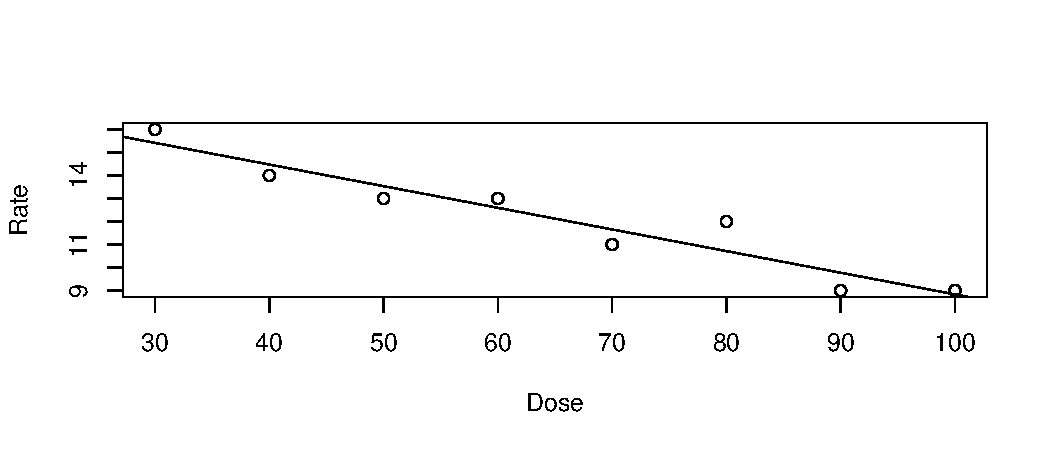
\includegraphics[width=\maxwidth]{figure/unnamed-chunk-22-1} 
\begin{kframe}\begin{alltt}
\hlstd{res} \hlkwb{=} \hlstd{y} \hlopt{-} \hlstd{(a} \hlopt{+} \hlstd{b} \hlopt{*} \hlstd{x)}
\hlkwd{plot}\hlstd{(x, res)}
\hlkwd{abline}\hlstd{(}\hlkwc{h} \hlstd{=} \hlnum{0}\hlstd{)}
\end{alltt}
\end{kframe}
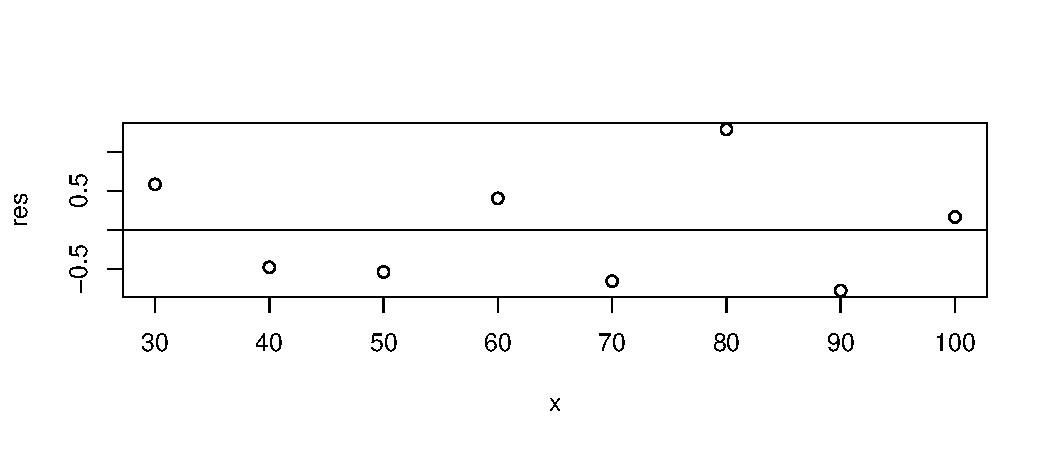
\includegraphics[width=\maxwidth]{figure/unnamed-chunk-22-2} 

\end{knitrout}

Comment: 
Based on both plots, it seems the linear fit is appropriate: The scatter plot shows a linear trend, and residual plot shows no observable pattern. \\


(c) 
Reverse the roles of $x$ and $y$, and then repeat the R commands.

\begin{knitrout}
\definecolor{shadecolor}{rgb}{0.969, 0.969, 0.969}\color{fgcolor}\begin{kframe}
\begin{alltt}
\hlstd{x}\hlkwb{=}\hlkwd{c}\hlstd{(}\hlnum{16}\hlstd{,}\hlnum{14}\hlstd{,}\hlnum{13}\hlstd{,}\hlnum{13}\hlstd{,}\hlnum{11}\hlstd{,}\hlnum{12}\hlstd{,}\hlnum{9}\hlstd{,}\hlnum{9}\hlstd{)}
\hlstd{y}\hlkwb{=}\hlkwd{c}\hlstd{(}\hlnum{30}\hlstd{,}\hlnum{40}\hlstd{,}\hlnum{50}\hlstd{,}\hlnum{60}\hlstd{,}\hlnum{70}\hlstd{,}\hlnum{80}\hlstd{,}\hlnum{90}\hlstd{,}\hlnum{100}\hlstd{)}
\hlkwd{cor}\hlstd{(x,y)}
\end{alltt}
\begin{verbatim}
## [1] -0.9533307
\end{verbatim}
\begin{alltt}
\hlstd{fit} \hlkwb{<-} \hlkwd{lm}\hlstd{(y}\hlopt{~}\hlstd{x)}
\hlstd{a}\hlkwb{=} \hlstd{fit}\hlopt{$}\hlstd{coefficients[[}\hlnum{1}\hlstd{]]}
\hlstd{a}
\end{alltt}
\begin{verbatim}
## [1] 182.1713
\end{verbatim}
\begin{alltt}
\hlstd{b}\hlkwb{=} \hlstd{fit}\hlopt{$}\hlstd{coefficients[[}\hlnum{2}\hlstd{]]}
\hlstd{b}
\end{alltt}
\begin{verbatim}
## [1] -9.663609
\end{verbatim}
\end{kframe}
\end{knitrout}

To predict dose from breathing rate, the LSR model is $\hat{y} = 182.1713  -9.663609x$,
where $y$ is dose and $x$ is breathing rate.

\end{solution}

\question 

The following data describes the relationship between obesity  measured as
    the percentage over ideal weight ($x$) and individual's response to pain 
    measured on a certain scale ($y$):
    \begin{center}\begin{tabular}{l|ccccc} $x$ & 89\% & 90\% & 75\% & 30\%
    & 51\% \\\hline $y$ & 2 & 3 & 4 & 4.5 & 5.5
    \end{tabular}
    \end{center}

\begin{parts}
\part Using R, produce a scatter plot, least squares regression line, correlation coefficient and residual plot.
 
\part Do the plots suggest that the linear fit is appropriate? If so, use the least squares line to predict the $y$-value for an $x$-value of $60\%$.
\end{parts}

\begin{solution}
(a) 
\begin{knitrout}
\definecolor{shadecolor}{rgb}{0.969, 0.969, 0.969}\color{fgcolor}\begin{kframe}
\begin{alltt}
\hlstd{x}\hlkwb{=}\hlkwd{c}\hlstd{(}\hlnum{89}\hlstd{,}\hlnum{90}\hlstd{,}\hlnum{75}\hlstd{,}\hlnum{30}\hlstd{,}\hlnum{51}\hlstd{)}
\hlstd{x}
\end{alltt}
\begin{verbatim}
## [1] 89 90 75 30 51
\end{verbatim}
\begin{alltt}
\hlstd{y}\hlkwb{=}\hlkwd{c}\hlstd{(}\hlnum{2}\hlstd{,}\hlnum{3}\hlstd{,}\hlnum{4}\hlstd{,}\hlnum{4.5}\hlstd{,}\hlnum{5.5}\hlstd{)}
\hlstd{y}
\end{alltt}
\begin{verbatim}
## [1] 2.0 3.0 4.0 4.5 5.5
\end{verbatim}
\begin{alltt}
\hlkwd{cor}\hlstd{(x,y)}
\end{alltt}
\begin{verbatim}
## [1] -0.7796686
\end{verbatim}
\begin{alltt}
\hlstd{fit} \hlkwb{<-} \hlkwd{lm}\hlstd{(y}\hlopt{~}\hlstd{x)}
\hlstd{a}\hlkwb{=} \hlstd{fit}\hlopt{$}\hlstd{coefficients[[}\hlnum{1}\hlstd{]]}
\hlstd{a}
\end{alltt}
\begin{verbatim}
## [1] 6.515211
\end{verbatim}
\begin{alltt}
\hlstd{b}\hlkwb{=} \hlstd{fit}\hlopt{$}\hlstd{coefficients[[}\hlnum{2}\hlstd{]]}
\hlstd{b}
\end{alltt}
\begin{verbatim}
## [1] -0.04052554
\end{verbatim}
\begin{alltt}
\hlstd{res} \hlkwb{=} \hlstd{y} \hlopt{-} \hlstd{(a} \hlopt{+} \hlstd{b} \hlopt{*} \hlstd{x)}
\hlkwd{plot}\hlstd{(x, res)}
\hlkwd{abline}\hlstd{(}\hlkwc{h} \hlstd{=} \hlnum{0}\hlstd{)}
\end{alltt}
\end{kframe}
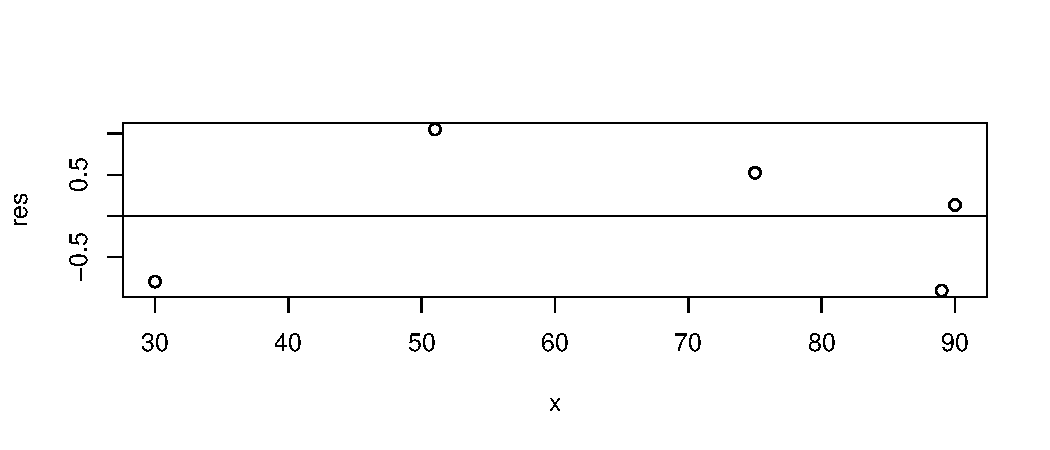
\includegraphics[width=\maxwidth]{figure/unnamed-chunk-24-1} 

\end{knitrout}
 
(b) 
The scatter plot suggests a linear fit. The residual plot may show a quadratic trend (which would  make the linear fit invalid), but it is hard to tell with only 5 data points. \\

IF the fit is valid, then
$\hat{y} = 6.515211 - (0.04052554)(60) \approx 4.08$.

\end{solution}
            
\end{questions}
\end{tutorial}
\end{document}

